\documentclass[fleqn,letterpaper,12pt,printwatermark=false]{memoir}
% memoir commands to define the text block geometry
\setulmarginsandblock{0.5in}{*}{*}
\setlrmarginsandblock{0.5in}{*}{*}
% put "extra" vertical space at the bottom of a page
\raggedbottom 

\usepackage{amsmath}
\usepackage{etoolbox} % for \ifblank etc
\usepackage{xparse} % for NewDocumentCommand et al.
\usepackage{enumitem}
\usepackage{transparent} % for \transparent, which I use in the watermark
\usepackage[slantedGreek]{mathpazo} \usepackage{helvet} % use Palatino et al.
\usepackage{booktabs} % prettier tables

\usepackage[]{xwatermark}
\newwatermark*[
    allpages,
    color=red!30,angle=45,
    scale=4,
    xpos=-10, ypos=0
]{%
    \transparent{0.4}dhasan example%
}

\usepackage{dashundergaps} % for \gap
\dashundergapssetup{
    teacher-mode=true, % set to true to show answers 
    gap-format=underline,
    teacher-gap-format=underline,
    gap-font={\sffamily},
    gap-numbers=true,
    gap-widen=true,
    gap-extend-percent=150, % note: making this too big might create errors
    gap-number-format=\,\textsuperscript{\normalfont(\thegapnumber)},
}

\usepackage{tcolorbox}
\tcbuselibrary{skins}
\tcbuselibrary{raster}

\usepackage{graphicx}
\graphicspath{ {../images/} }
\begin{document}

\newcommand{\myClassName}{Pre-AP Algebra 2}
\newcommand{\myUnitNumber}{1}
\newcommand{\myUnitTitle}{Introduction to Functions}
\newcommand{\myLessonNumber}{1}
\newcommand{\myLessonTitle}{Relations and Functions}


\copypagestyle{myPagestyle}{empty}


\newcommand{\myFooterSize}{\footnotesize}
\makeoddfoot{myPagestyle}{{}}{\myFooterSize{\thepage{}~of~\pageref*{xwmlastpage}}}{\myFooterSize\thetitle}
\makeevenfoot{myPagestyle}{{}}{\myFooterSize{\thepage{}~of~\pageref*{xwmlastpage}}}{\myFooterSize\thetitle}

%
% A command to change the appearance of the cognitive verb 
% in the objectives.
%
\newcommand{\myCognitiveVerb}[1]{\textcolor{blue}{\textbf{#1}}}

%
% Terminology explanation:
%
% "unit" refers to the Algebra 2 unit being taught.
% "section" refers to the section within the unit being taught.
% "heading" refers to the headings in this document (Objectives, Example, ...)
%
\NewDocumentCommand{\myUnitSectionNumberFont}{}{\sffamily\bfseries\HUGE}
\NewDocumentCommand{\myUnitNameFont}{}{\sffamily\large}
\NewDocumentCommand{\mySectionNameFont}{}{\sffamily\bfseries\huge}
\NewDocumentCommand{\myHeadingFont}{}{\sffamily\bfseries\Large}


%
% #1 is the fill-in text
%
\NewDocumentCommand{\myFillInBlank}{m}{%
    \,%
    \gap[u]{#1}%
    \,%
}


% Definition for the LESSON HEADER + OBJECTIVES
%
% #1 : optional unit name
% #2 : optional unit/section number
% #3 : mandatory title
%
\NewDocumentEnvironment{myNotesHeader}{oom}{
    \title{#3}
    \begin{flushleft}
        \IfValueT{#2}{{\myUnitSectionNumberFont#2}}
        \hfill\;\;
        \begin{minipage}[b]{0.75\textwidth}
            \begin{flushright}
                \IfValueT{#1}{
                    {\myUnitNameFont#1}\\ \vspace{0.75em}
                }
                {\mySectionNameFont#3}
            \end{flushright}
        \end{minipage}
        \hrule
    \end{flushleft}
    \noindent{\myHeadingFont Objectives:}
    \begin{enumerate}[label=\arabic*)]
}{
    \end{enumerate}
}


% Definitions related to the VOCABULARY TABLE
%
\newenvironment{myVocabulary}{
    {\noindent{\myHeadingFont Vocabulary:}}\vspace{1em}

    \begin{tabular}{ll}
        \toprule
            \emph{word} & \emph{meaning} \\ 
        \midrule
}{
    \bottomrule
    \end{tabular}
    \vspace{1em}
}

\newcommand{\myVocabularyWord}[2]{%
{\textcolor{blue}{\textbf{#1}}} & #2 \\
}


% Definitions related to an INTRODUCTION
%
\newenvironment{myIntroduction}{
    {\noindent{\myHeadingFont Introduction:}}\vspace{1em}

    \setlength{\leftskip}{3cm}
}{
    \setlength{\leftskip}{0pt}
}


% Definition related to KEY CONCEPTS
%
% #1 : the key concept (which appears as a tcolorbox title)
%
\NewDocumentEnvironment{myKeyConcepts}{ O{Key Concepts:} }{
    \begin{tcolorbox}[
        title=#1, fonttitle=\myHeadingFont,
        coltitle=black, 
        colbacktitle=black!25!yellow, 
        colframe=black!50!yellow,
        colback=white!70!yellow,
        boxrule=2pt, 
        ]
}{
    \end{tcolorbox}
}


% Definition related to EXAMPLES
%
% #1 Optional example number 
% #2 A statement of the example problem.
% #3 How much empty vertical space to leave for the example box.
%
\NewDocumentCommand{\myExample}{omm}{%
    \begin{tcolorbox}[
        enhanced,
        sharp corners, 
        colback=white,
        boxrule=0pt,
        borderline={0.5pt}{0pt}{black,dashed},
        ]
        {\myHeadingFont Example\IfValueT{#1}{{ #1}}:}
        #2
        \tcblower
        \vspace{#3}
    \end{tcolorbox}
}

% Definitions related to PROBLEMS

% A counter to number the problems in the guided notes.
\newcounter{MyProblemCounter}
\setcounter{MyProblemCounter}{1}
\newcommand{\useMyProblemCounter}{\theMyProblemCounter\stepcounter{MyProblemCounter}}

% an environment for two adjacent problems
%
% #1 : directions for all the problems
% #2 : vertical height of the problem boxes
% #3 : details for problem 1
% #4 : details for problem 2
%
\newenvironment{myProblems2}[4]{%
    \noindent
    {\myHeadingFont Practice:}\hspace{0.5em}#1\nopagebreak%
    \begin{tcbraster}[%
        raster equal height,%
        raster columns=2,%
        raster column skip=0.5mm,%
        raster row skip=0.5mm,%
        raster every box/.style={%
            enhanced,%
            sharp corners,%
            colback=white,%
            coltitle=black, colbacktitle=black!10!white,%
            boxrule=0pt, borderline={0.5pt}{0pt}{black},%
            title={\texttt\useMyProblemCounter},%
            },%
        ]%
        \begin{tcolorbox}[attach boxed title to top left]
            #3
            \tcblower\vspace{#2}
        \end{tcolorbox}
        \begin{tcolorbox}[attach boxed title to top right]
            #4
            \tcblower
        \end{tcolorbox}%
}{%
    \end{tcbraster}
}

% an environment for 4 adjacent problems
%
% #1 : directions for all the problems
% #2 : vertical height of the problem boxes
% #3 : details for problem 1
% #4 : details for problem 2
% #5 : details for problem 3
% #6 : details for problem 4
%
\newenvironment{myProblems4}[6]{%
    \noindent
    \textbf{\myHeadingFont Practice:}\hspace{0.5em}#1\nopagebreak%
    \begin{tcbraster}[%
        raster equal height,%
        raster columns=2,%
        raster column skip=0.5mm,%
        raster row skip=0.5mm,%
        raster every box/.style={%
            enhanced,%
            sharp corners,%
            colback=white,%
            coltitle=black, colbacktitle=black!10!white,%
            boxrule=0pt, borderline={0.5pt}{0pt}{black},%
            title={\texttt\useMyProblemCounter},%
            },%
        ]%
        \begin{tcolorbox}[attach boxed title to top left]
            #3
            \tcblower\vspace{#2}
        \end{tcolorbox}
        \begin{tcolorbox}[attach boxed title to top right]
            #4
            \tcblower
        \end{tcolorbox}%
        \begin{tcolorbox}[attach boxed title to bottom left]
            #5
            \tcblower
        \end{tcolorbox}%
        \begin{tcolorbox}[attach boxed title to bottom right]
            #6
            \tcblower
        \end{tcolorbox}%
}{%
    \end{tcbraster}
}
\pagestyle{myPagestyle}

\checkandfixthelayout
\setlist{labelindent=\parindent,leftmargin=*,itemsep=0.025em,label=$\circ$}

% ---------------------HEADER------------------------------
\begin{myNotesHeader}
    \item \myCognitiveVerb{find} the domain and range of a relation
    \item \myCognitiveVerb{determine} if a relation is a function
\end{myNotesHeader}

\begin{myVocabulary}
    \myVocabularyWord{relation}
        {
            a set of relationships between inputs and outputs
            (usually $x$'s and $y$'s)
        }
        \myVocabularyWord{function}
        {
            a special kind of relation
        }
        \myVocabularyWord{domain}
        {
            the set of all the inputs in a relation 
            (usually the $x$'s)
        }
        \myVocabularyWord{range}
        {
            the set of all the outputs in a relation 
            (usually the $y$'s)
        }
        \myVocabularyWord{vertical}
        {
            something that goes up and down
        }
        \myVocabularyWord{ordered pairs}
        {
            pairs of $x$'s and $y$'s For example, $(-2,13)$ is an ordered pair.
        }
\end{myVocabulary}

% ---------------------LESSON 1------------------------------
\begin{myLesson}[][1]
    A relation is a set of inputs and their associated outputs.
    To each input there is a corresponding output.
    Usually (but not always) we use $x$ for the inputs
    and $y$ for the outputs.
    In this case, we say that a relation is 
    a set of $x$'s and their corresponding $y$'s.

    There are several ways to specify a relation:
    \begin{itemize}
        \item {\bfseries\itshape ordered pairs}: 
        a set that lists the inputs and corresponding outputs as ordered pairs
        \item {\bfseries\itshape tables}: 
        a table of all the inputs and corresponding outputs
        \item {\bfseries\itshape mappings}: 
        diagrams that use arrows to connect inputs to their corresponding outputs
        \item {\bfseries\itshape graphs}: 
        graphs that plot all the ordered pairs in a 2-D grid 
        (either as a collection of points or, more often, as a curve of infinitely many points)
    \end{itemize}

    \begin{myWorkedExample}{
            Represent the relation
            \(
                \{ (1,2), (3,2), (5,-2), (1,-3) \}
            \)
            as a table, mapping, and graph.
        }
        As an intput-output table:

        \begin{center}
        \begin{tabular}{cc}
            \toprule
            \emph{inputs} & \emph{outputs} \\
            \midrule
            1 & 2\\
            3 & 2\\
            5 & -2\\
            1 & -3\\
            \bottomrule
        \end{tabular}
        \end{center}

        As a mapping from inputs to outputs:

        \begin{center}
            \(
                1 \longrightarrow 2
            \)\\
            \(
                3 \longrightarrow 2
            \)\\
            \(
                5 \longrightarrow -2
            \)\\
            \(
                1 \longrightarrow -3
            \)
        \end{center}
    
        As a graph:

        \begin{center}
            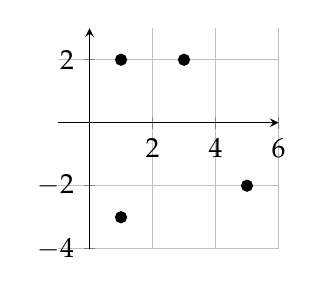
\begin{tikzpicture}
                \begin{axis}[
                    width=2in,
                    grid=both,
                    axis x line = middle,axis y line = middle,
                    axis equal image,
                    % minor tick num=1,
                    xtick distance = 2, ytick distance = 2,
                    xmin = -1, xmax=6,
                    ymin = -4, ymax=3,
                    ]
                    \addplot[
                        only marks,
                        mark=*,
                        % mark size = 0.15cm,
                        ] coordinates { (1,2) (3,2) (5,-2) (1,-3) };
                \end{axis}
            \end{tikzpicture}
        \end{center}
    \end{myWorkedExample}

    The \emph{domain} of a relation is the set of all the inputs.
    It's all the inputs of the ordered pairs.
    Or it's all the inputs in the table or the mapping.
    Or it's all the inputs coordinates in the graph.
    Since we usually use the variable $x$ for inputs,
    \begin{myLessonBox}[3in]
        The {\bfseries\itshape domain} is the set of all the $x$'s.
    \end{myLessonBox}

    The \emph{range} of a relation is the set of all the outputs.
    It's all the outputs of the ordered pairs.
    Or it's all the outputs in the table or the mapping.
    Or it's all the outputs coordinates in the graph.
    Since we usually use the variable $y$ for outputs,
    \begin{myLessonBox}[3in]
        The {\bfseries\itshape domain} is the set of all the $y$'s.
    \end{myLessonBox}
\end{myLesson}

% ---------------------CONCEPT 1------------------------------
\begin{myKeyConcepts}[To find the domain and range of a relation\dots]
    Follow these steps:
    \setlist{labelindent=\parindent,}
    \begin{enumerate}
        \item {\bfseries\itshape Write down} all the inputs ($x$ values).
        \item The {\bfseries\itshape domain} is those values \emph{without any duplicated values}.
        \item {\bfseries\itshape Write down} all the outputs ($y$ values).
        \item The {\bfseries\itshape range} is those values \emph{without any duplicated values}.
    \end{enumerate}
\end{myKeyConcepts}

\myExample{
    Find the domain and range of this relation:
    \(
        \{ (1,2), (5,6), (3,4) \}
    \)
}{1in}

\myExample{
    Find the domain and range of this relation:
    \begin{center}
        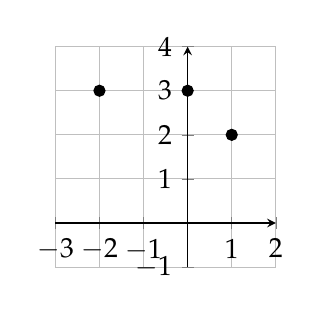
\begin{tikzpicture}
            \begin{axis}[
                width=2in,
                grid=both,
                axis x line = middle,axis y line = middle,
                axis equal image,
                xtick distance = 1, ytick distance = 1,
                xmin = -3, xmax=2,
                ymin = -1, ymax=4,
                ]
                \addplot[
                    only marks,
                    mark=*,
                    % mark size = 0.15cm,
                    ] coordinates { (1,2) (-2,3) (0,3) };
            \end{axis}
        \end{tikzpicture}
    \end{center}
}{1in}

% ---------------------LESSON 2------------------------------
\begin{myLesson}[][2]
    A function is a special kind of relation
    where each input ($x$ value) has one {\bfseries\itshape and only one} output ($y$ value).
    It is possible that two different inputs will have the same output,
    but for functions,
    a single input will never have more than one output.
\end{myLesson}

% ---------------------CONCEPT 2------------------------------
\begin{myKeyConcepts}[To determine of a relation consisting of a set of points is a function\dots]
    Follow these steps:
    \setlist{labelindent=\parindent,}
    \begin{enumerate}
        \item {\bfseries\itshape Write down} all the inputs ($x$ values).
        \item For each of the input values, {\bfseries\itshape write down} all of its outputs ($y$ values).
        To do this, you will have to look through all the points in the relation that have 
        that particular input value.
        \item {\bfseries\itshape Ask} ``Are any inputs with more than one output?''
        \item If the answer to that question is yes, 
        then the relation {\bfseries\itshape is not a function}.
        Otherwise, the relation {\bfseries\itshape is a function}.
    \end{enumerate}
\end{myKeyConcepts}

\myExample{
    Determine if this relation is a function. Explain your answer.
    \(
        \{ (1,2), (5,6), (3,4), (3,2) \}
    \)
}{1in}

\myExample{
    Determine if this relation is a function. Explain your answer.
    \begin{center}
    \begin{tabular}{cc}
            \toprule
            \emph{inputs} & \emph{outputs} \\
            \midrule
            1 & 2\\
            -5 & 3\\
            5 & -2\\
            1 & -3\\
            \bottomrule
    \end{tabular}
    \end{center}
}{1in}


\myExample{
    Find the domain and range of this function, and determine if it is a function. 
    Explain your answer.
    \begin{center}
    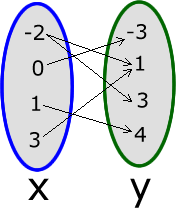
\includegraphics[width=2in]{domain-range-mapping.png}
    \end{center}
}{2.5in}

% ---------------------CONCEPT 3------------------------------
\begin{myKeyConcepts}[To determine of a relation represented as the graph is a function\dots]
    Follow these steps:
    \setlist{labelindent=\parindent,}
    \begin{enumerate}
        \item {\bfseries\itshape Look closely} at the graph.
        \item Are there any vertical lines 
        that {\bfseries\itshape intersect the graph in more than one place?}
        \item If so, 
        the relation {\bfseries\itshape is not a function}.
        Otherwise, the relation {\bfseries\itshape is a function}.
    \end{enumerate}

    This is called the {\bfseries\itshape Vertical Line Test}. 
\end{myKeyConcepts}

\myExample{
    Determine if this relation is a function. Explain your answer.
    \begin{center}
        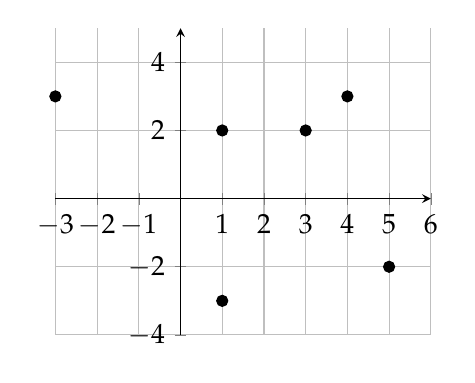
\begin{tikzpicture}
            \begin{axis}[
                width=2.5in,
                grid=both,
                axis x line = middle,axis y line = middle,
                % axis equal image,
                % minor tick num=1,
                xtick distance = 1, ytick distance = 2,
                xmin = -3, xmax=6,
                ymin = -4, ymax=5,
                ]
                \addplot[
                    only marks,
                    mark=*,
                    % mark size = 0.15cm,
                    ] coordinates { (-3,3) (1,2) (3,2) (5,-2) (1,-3) (4,3) };
            \end{axis}
        \end{tikzpicture}
    \end{center}
}{1in}


\myExample{
    Are these functions? Explain why or why not.
    \begin{center}
        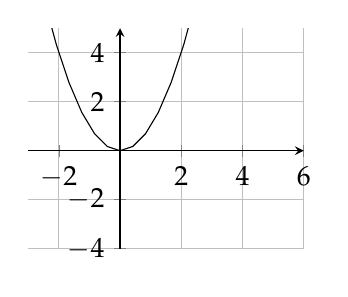
\begin{tikzpicture}
            \begin{axis}[
                width=2in,
                grid=both,
                axis x line = middle,axis y line = middle,
                % axis equal image,
                % minor tick num=1,
                % xtick distance = 1, ytick distance = 2,
                xmin = -3, xmax=6,
                ymin = -4, ymax=5,
                ]
                \addplot[no marks] expression { x^2 };
            \end{axis}
        \end{tikzpicture}
        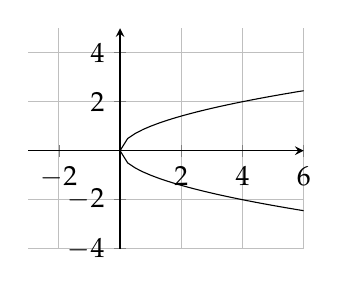
\begin{tikzpicture}
            \begin{axis}[
                width=2in,
                grid=both,
                axis x line = middle,axis y line = middle,
                % axis equal image,
                % minor tick num=1,
                % xtick distance = 1, ytick distance = 2,
                xmin = -3, xmax=6,
                ymin = -4, ymax=5,
                ]
                \addplot[no marks,domain=0:6] expression { sqrt(x) };
                \addplot[no marks,domain=0:6] expression { -sqrt(x) };
            \end{axis}
        \end{tikzpicture}
        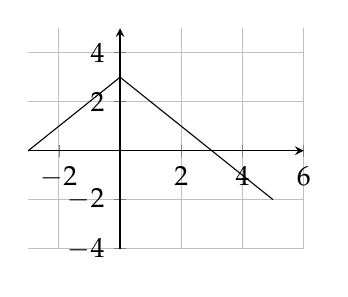
\begin{tikzpicture}
            \begin{axis}[
                width=2in,
                grid=both,
                axis x line = middle,axis y line = middle,
                % axis equal image,
                % minor tick num=1,
                % xtick distance = 1, ytick distance = 2,
                xmin = -3, xmax=6,
                ymin = -4, ymax=5,
                ]
                \addplot[no marks] expression { -abs(x) + 3 };
            \end{axis}
        \end{tikzpicture}
        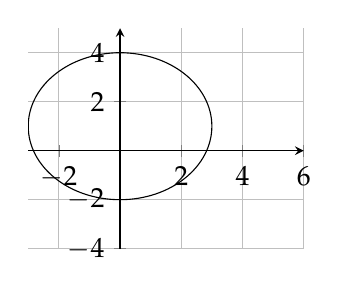
\begin{tikzpicture}
            \begin{axis}[
                width=2in,
                grid=both,
                axis x line = middle,axis y line = middle,
                % axis equal image,
                % minor tick num=1,
                % xtick distance = 1, ytick distance = 2,
                xmin = -3, xmax=6,
                ymin = -4, ymax=5,
                ]
                \draw (axis cs:0,1) circle [radius=3];
            \end{axis}
        \end{tikzpicture}
    \end{center}
}{3in}

% \begin{myProblems2}%
%     {Factor the following monomials into prime factors.}%
%     {2in}%
%     %
%     {\( 32x^2 \)}
%     {\( 8 x^3y^2z \)}
% \end{myProblems2}
  


\end{document}